% $Id$

\chapter{Quick Start Tutorial}

This chapter provides a quick start tutorial for using CUTS. After 
reading this chapter, you will have a basic understanding of how to:
\begin{enumerate}
  \item Model application behavior and workload.

  \item Generate a test system model the constructed model.

  \item Execute the system in your target environment.

  \item Collect and analyze test results (COMING SOON).
\end{enumerate}

In this tutorial, you will be measure and analyze the service time 
a simple server component. This tutorial assumes you have basic 
understanding of the Generic Modeling Environment (GME), CoSMIC/\-PICML, 
and the CORBA Component Model (CCM). This tutorial targets the 
Component Integrated ACE ORB (CIAO) middleware\footnote{CIAO is 
an open-source implementation of the CCM, and is freely available 
for download at the following location: \url{www.dre.vanderbilt.edu/CIAO}.}. 
Although this tutorial targets CIAO, the experience gained can be 
applied to other architectures that CUTS supports.

\section{Modeling Behavior and Workload}
\label{sec:quickstart-modeling}

Using GME, open the following file: 
\begin{lstlisting}
(*@\texttt{\$(CUTS\_ROOT)/examples/PICML/GettingStarted.xme}@*)
\end{lstlisting}
This model contains the structure of the client/\-server application, and 
is usually the starting point for using CUTS within PICML. 
Currently, application behavior and workload is modeled in the \texttt{Behavior}
aspect of a component's interface definition in PICML. The components in the model
located at:
\begin{lstlisting}
(*@\texttt{GettingStarted/InterfaceDefinitions/GettingStarted/GettingStarted}@*)
\end{lstlisting}
already contain model elements for its input/\-output ports. What remains is associating
the correct behavior and workload with these input/\-output ports for emulation
purposes. First, let's add behavior and workload to the client component by 
assuming the client component should periodically send an event to the server.
Please complete the following steps (elements will be automatically be generated
as well):
\begin{enumerate}
  \item Add a \texttt{PeriodicEvent} model element to the active model and 
  set its name to \texttt{periodicPing} and its \texttt{Hertz} attribute to 
  10 (\textit{i.e.}, 10 events/sec). 
  
  \item Insert an \texttt{InputAction} element, change its name to 
  \texttt{periodicPing}, and connect the \texttt{PeriodicEvent} to 
  the \texttt{InputAction}.

  \item Insert an \texttt{OutputAction}, connect it with the \texttt{State}.

  \item Connect the final \texttt{State} with the originating \texttt{InputAction},
  \textit{i.e.}, \texttt{periodicPing}, to signify end of the behavior.
\end{enumerate}
Figure~\ref{fig:gettingstarted-client-behavior} illustrates the complete behavior 
model of the client in PICML, which is implemented in the previous steps.
\begin{figure}[htbp]
  \centering
  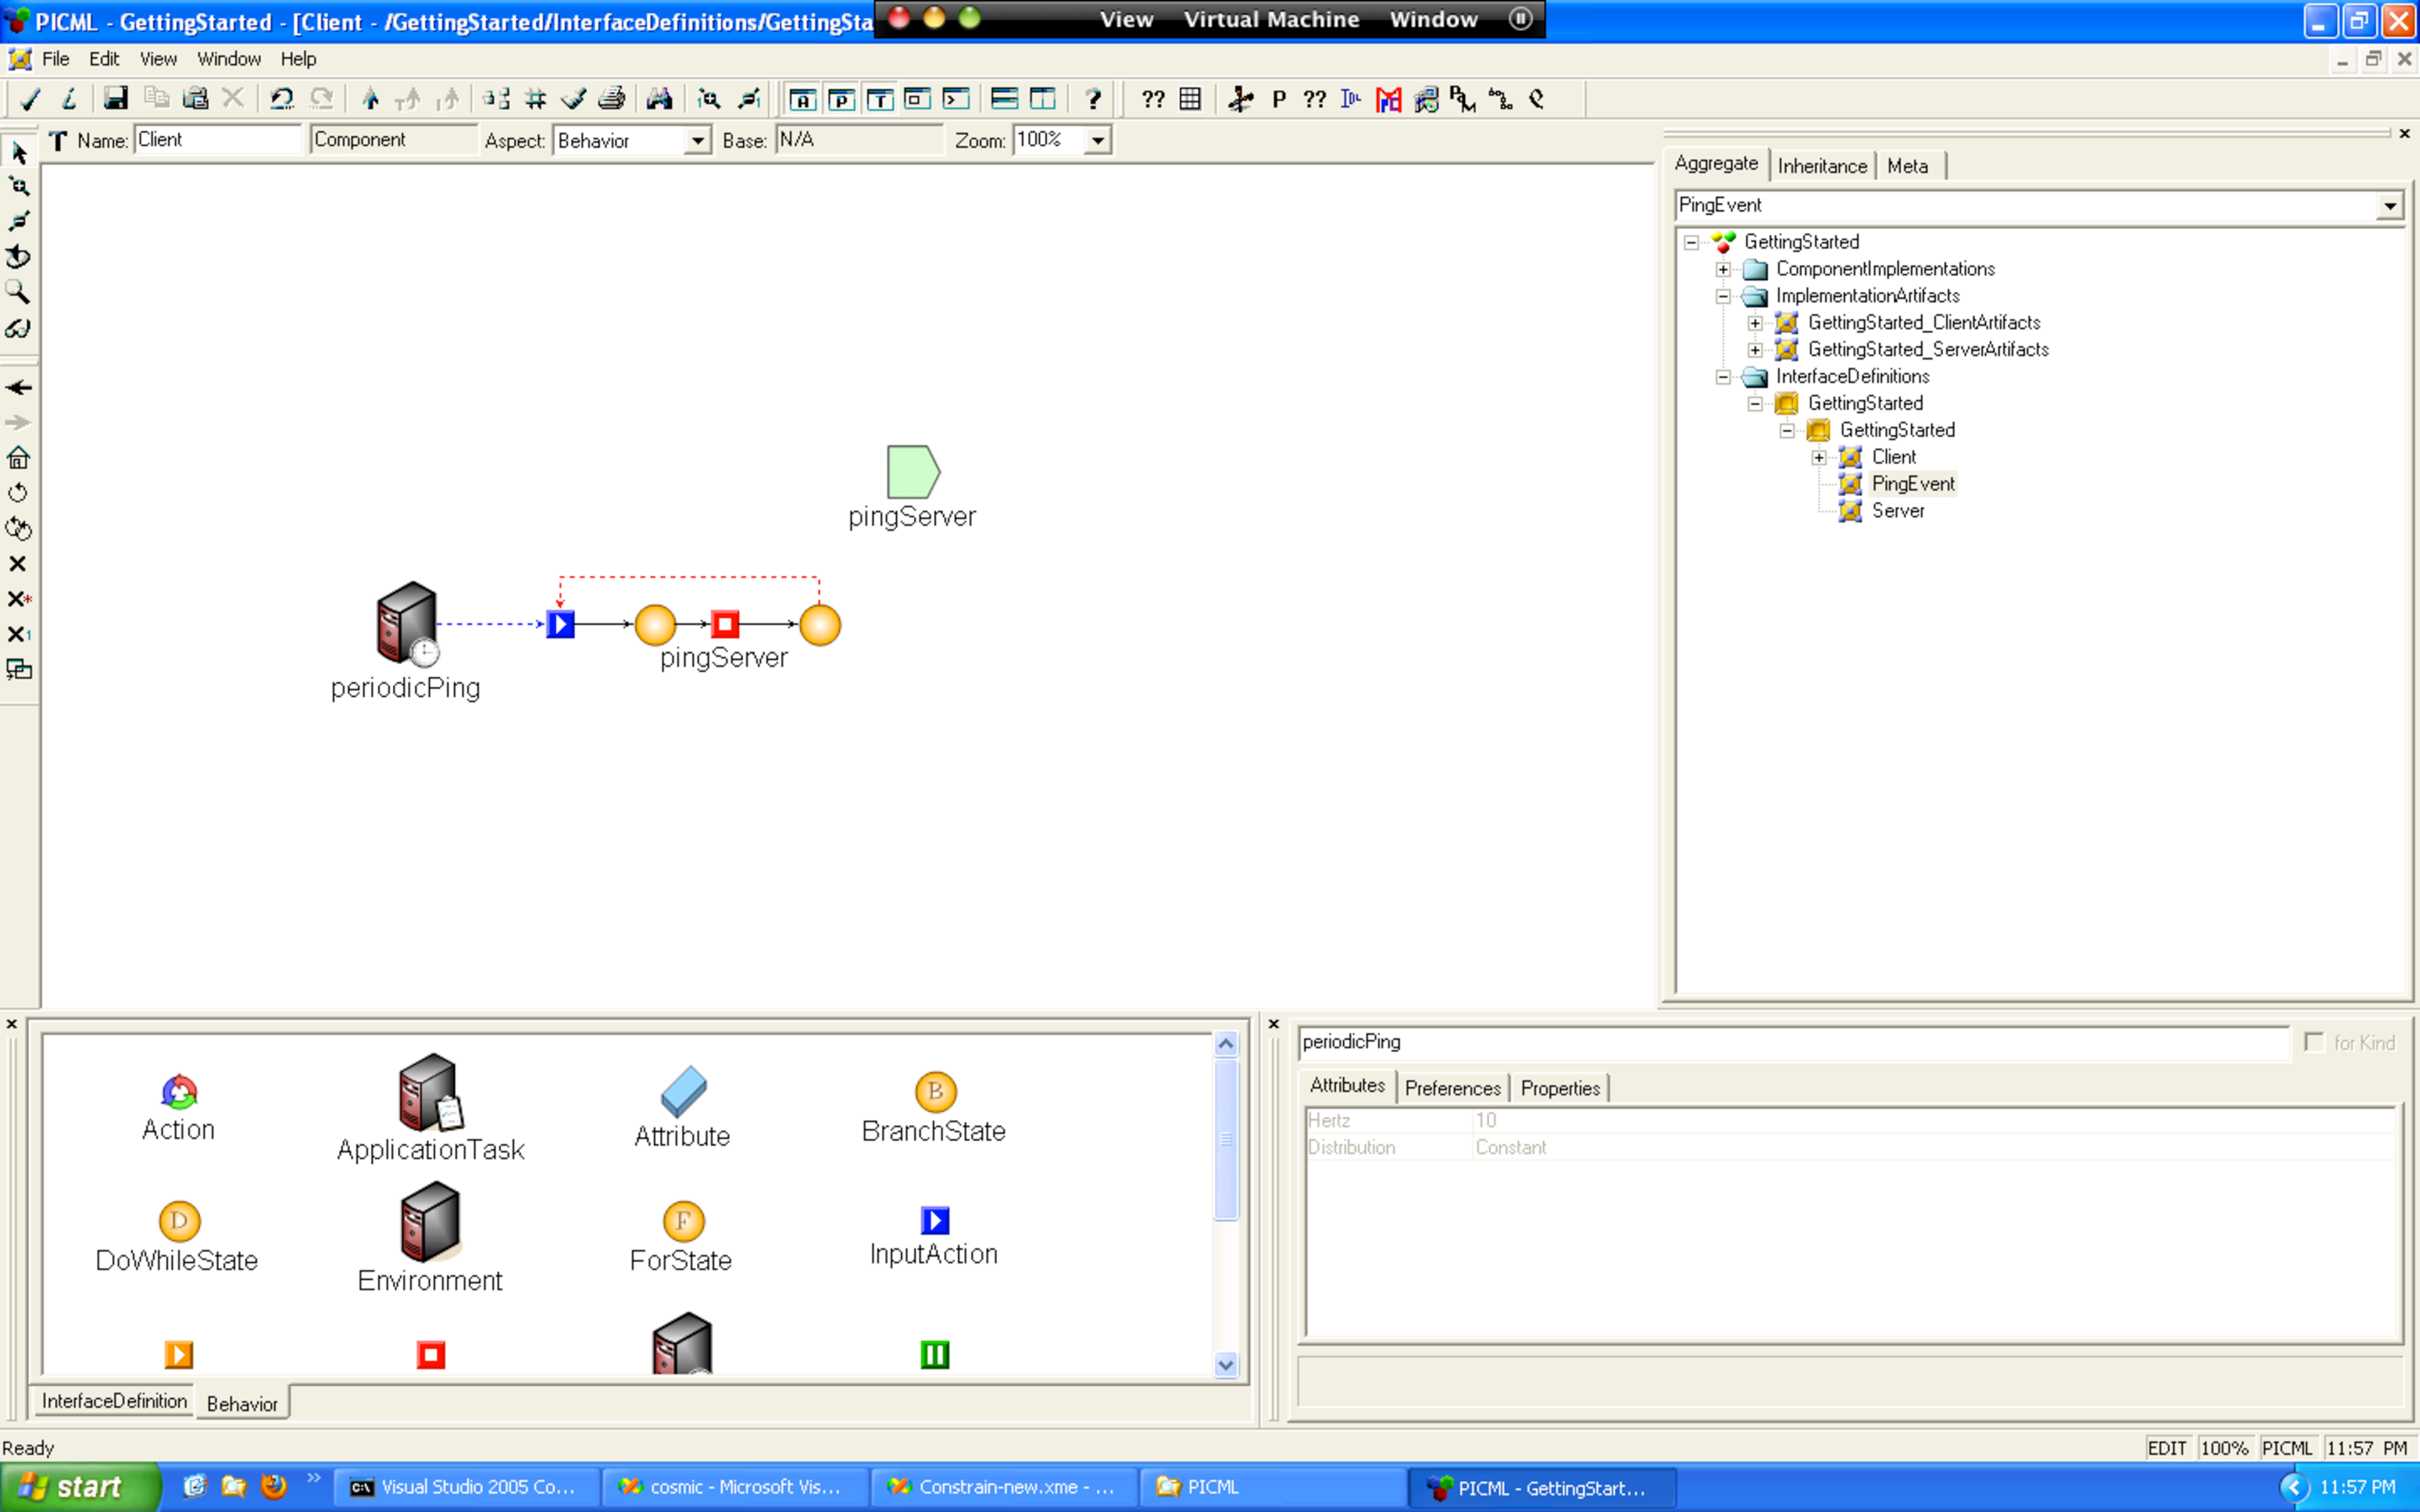
\includegraphics[scale=0.3]{gettingstarted-client-behavior-new.pdf}
  \caption{Client behavior model in PICML for CUTS emulation.}
  \label{fig:gettingstarted-client-behavior}
\end{figure}

Since you will need to collect performance metrics from the server
component, its behavior/workload has already been completed. You,
however, will learn how to add the necessary elements to the model
to collect performance metrics in later chapters.

\section{Generating Test System Implementation}
\label{sec:quickstart-generation}

After modeling the behavior and workload, the next step is to 
generate source code from the model. This will enable emulation 
of the test system on its target architecture. To generate source 
code from the model, launch the CUTS interpreter and excute the 
following steps (also illustrated in Figure~\ref{fig:gettingstarted-generation}):
\begin{enumerate}
  \item Select \texttt{Generate component implementation} radio button;
  \item Enter the target output directory;
  \item Select \texttt{Component Integrated ACE ORB (CIAO)} in the listbox;
  \item Click the \texttt{OK} button.
\end{enumerate}
\begin{figure}[htbp]
  \centering
  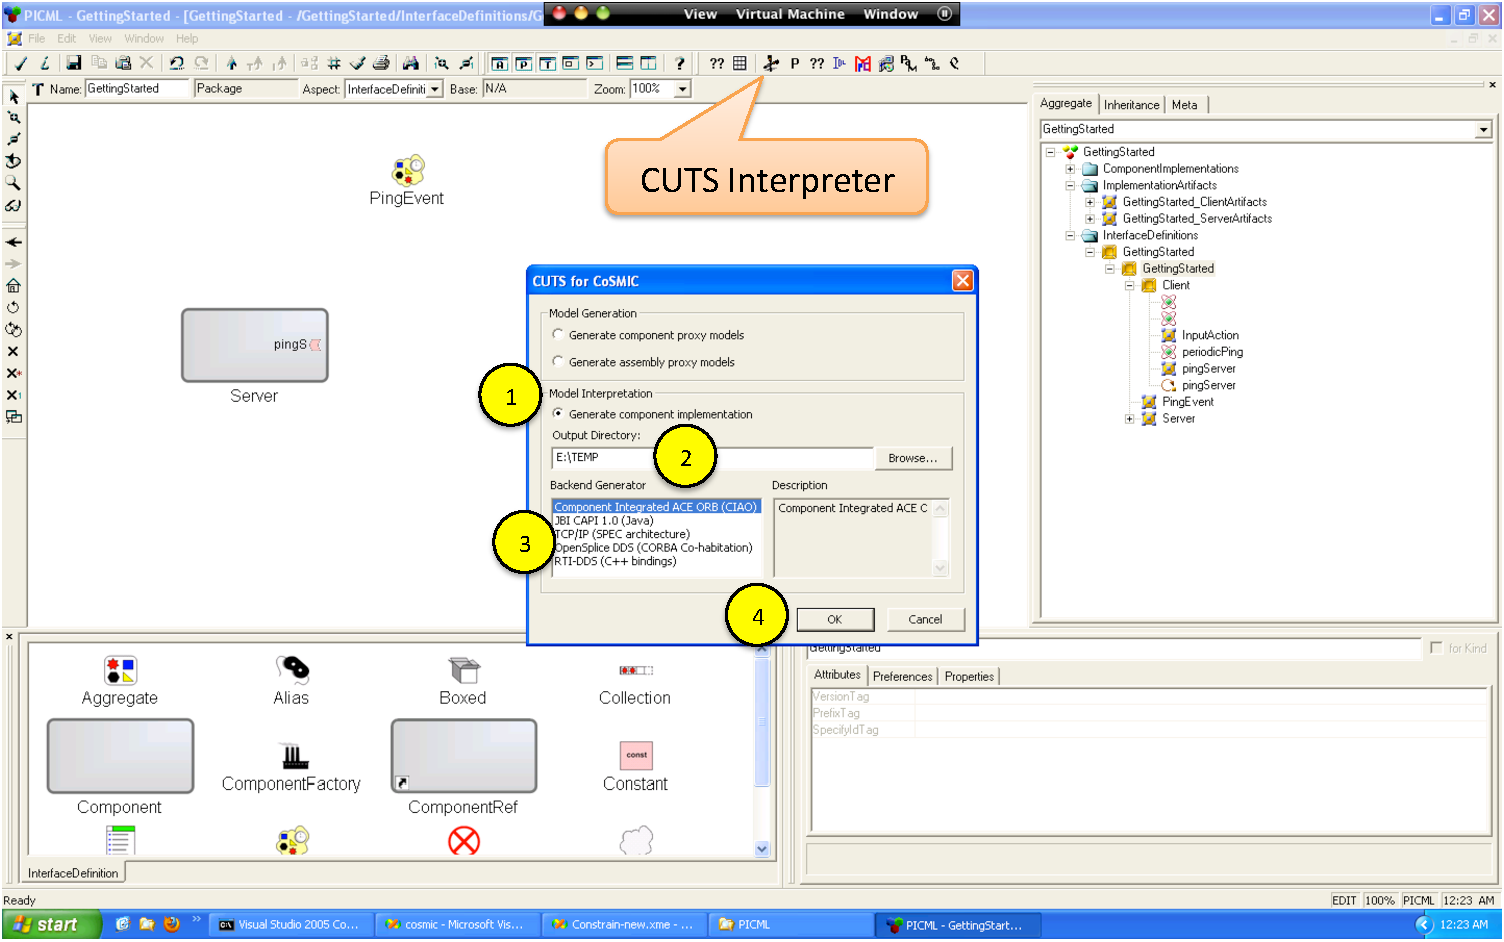
\includegraphics[scale=0.6]{gettingstarted-generation.pdf}
  \caption{Walkthrough of the steps for generating source code from
  CBML/WML models in CUTS.}
  \label{fig:gettingstarted-generation}
\end{figure}

Once the CUTS interpreter finishes generating source code, the IDL and CIDL 
files need to be generated in order to compile the source code. These files 
are created by the IDL Generator and CIDL Generator interpreters, respectively, 
provided with CoSMIC~\footnote{Please ensure to generate the IDL and CIDL 
files in the same directory as the source code previously generated 
from the model.}. Finally, there will be a \texttt{GettingStarted.mwc} 
file (its name may be different) located in the output directory selected 
for source code generation. This is a Makefile, Project and Workspace Creator 
(MPC) workspace file that contains all the necessary information to sucessfully 
compile the generated source code. Use \texttt{GettingStarted.mwc} to generate 
the appropriate workspace and then compile it.

\section{Executing in Target Environment}
\label{sec:quickstart-execution}

One design goal of CUTS is to (re)use the same infrastruture used in the 
target environment. The \texttt{GettingStarted.xme} example uses the Deployment 
And Configuration Engine (DAnCE), which is included with CIAO's standard 
distribution, to deploy the test system. To deploy the CUTS stock quoter 
example, use the following steps~\footnote{CUTS has a distributed testing
framework that simplifies many of the complexities associated with running
distributed system tests. We will cover the CUTS testing framework in later
chapters}:
\begin{enumerate}
  \item Generate the flat deployment plan descriptors from the 
  \texttt{GettingStarted}  model. You can find instructions on generating 
  the flat deployment plan in the original stock quoter tutorial included 
  with CoSMIC.
  
  \item Use DAnCE to deploy the GettingStarted.cdp. The original stock 
  quoter tutorial in CoSMIC has instructions on how to deploy a solution. 
  Be sure, however, to update the \texttt{nodemap.dat} file to the appropriate
  hosts and their location.
\end{enumerate}
When the CUTS version of the GettingStarted example is deployed, the test
manager will periodic collect log messages from each host/\-client, and 
insert them into a SQLite database for postprocessing.

\section{Analyzing Test Results}
\label{sec:quickstart-analysis}

Collecting and analyzing tests results in CUTS requires more in-depth
knowledge of CUTS and its other toolsets. For these reasons, the Quick
Start Tutorial does not cover this aspect of CUTS.

%\begin{tabular}{p{0.5in}p{6.0in}}
%\modeldef{modeling/action.pdf}{Action}{This is the action icon.}

%\end{tabular}
